To predict punctuations in unformatted text, we use two different models: a lexical model, which is based on lexical features, and an acoustic model, which is based on prosodic features.
For our approach we used a deep learning approach using the deep learning framework \emph{Caffe}\footnote{http://caffe.berkeleyvision.org/}. 
In this chapter we describe how we predict the position of periods and commas in unpunctuated text using lexical features.

\subsection{Training instance generation}
For training our lexical model we took the \texttt{.xml} files of the TED talks and the Wikipeida files.
To generate the training instance, which are then used to train our neural network with \emph{Caffe}, we have to preprocess the data.
An overview of the individual steps from obtaining the training instances out of the input files, is shown in Figure~\ref{fig:overview_lexical}.
\begin{figure}[ht]
    \centering
    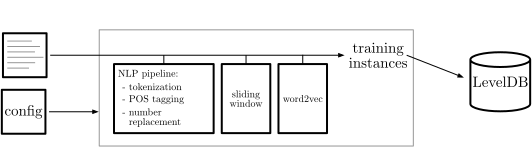
\includegraphics[width=0.7\textwidth]{img/overview_lexical.pdf}
    \caption{TODO}
    \label{fig:overview_lexical}
\end{figure}

In a first step the plain text from the input files is extracted.
The input text is formatted, i.e., it contains all kinds of punctuation marks.
Therefore, we can create a gold standard out of it.
We use the following two classes: \textsc{Period} and \textsc{Comma}.
The class \textsc{Period} is mapped to the following characters: ``;'', ``.'', ``!'' and ``?''.
The characters ``,'', ``:'' and ``-'' are mapped to the class \textsc{Comma}.

Having the input text, the first step is to tokenize it.
Afterwards, a sliding window is used to split the input text into smaller parts and to create our training instances.
An example, which shows how the sliding window works, is shown in Figure~\ref{fig:sliding_window}.
\begin{figure}[ht]
    \centering
    
\includegraphics[width=0.8\textwidth]{img/sliding_window.pdf}
    \caption{Sliding window of window size 5. The class of the created window, is determined by the punctuation after the third word. TODO}
    \label{fig:sliding_window}
\end{figure}
The size of the window is determined by a \texttt{config} file.
The \texttt{config} file stores different parameter, which are used during the process of generating the training instances.
Having those \texttt{config} files makes it easy to generate different kind of training instances and therefore to evaluate different kid of configurations.
The window size directly defines the size of the training instance.
The label of a training instance is determined by whether there is a punctuation at a certain position or not.
This position is also defined in the \texttt{config} file and is called punctuation position.
In the example in Figure~\ref{fig:sliding_window} we have a punctuation position of 3.
If there is no punctuation at this position the label of the training instance would be 0 (stands for class \textsc{None}), if there is one character of the class \textsc{Comma}, it would be 1, and if it is a character of the class \texttt{Period}, the label would be 2.

After we divide the sentences into training instances, we convert each word into a distributed word representation.
Thus, we obtain a representation of our training instances, which \emph{Caffe} can handle.
We use the distributed word representation \emph{word2vec}\footnote{\url{https://code.google.com/archive/p/word2vec/}}.
\emph{word2vec} is TODO~\cite{Mikolov1, Mikolov2, Mikolov3}.
The final model we used for our distributed word representation was trained on a Google news dataset.
The model contains 300-dimensional word vectors for 3 million different words and phrases.
Since not every word exists in the trained model, we use the word vector representing \texttt{this} for unknown words.
We think that most of the unknown words are proper names, which can be replaced with \texttt{this} without changing the meaning and structure of the whole sentence.

We also figured out that the trained model only contains the number \emph{1} and a few more of the most common numbers instead of all numbers. \todo{Check whether only 1 is in the word vector or whether numbers like 12 and 5 are also contained}
That is why we replace any number with \emph{1}.

The representation for each word in an instance is inserted into one row of the feature matrix, e.g. for a sliding window size of 5 you get the matrix of 5x300 for each instance.

Besides the distributed word representation we also examined Part of Speech (POS) tags as features.
We used the nltk POS tagger to identify the POS tags with the whole text as input.
The tagger distinguishes between 35 different POS tags.
These are too specific for our purpose, so we reduced them into 14 different categories.
For example we combined CD and LS to a more generic category \emph{numeral}.
The nltk tagger predicts more than one tag per word, so one word can have multiple tags (even after reducing the tag categories).
To allow the existence of multiple tags in our feature matrix, we used the following representation:
We create one flag per POS category which has the value 1 if the word belongs to this category and 0 otherwise.

There are two possibilities to include them.
On the one hand it is possible to append all flags at the end to word vector representations.
On the other hand an extra channel with the flags can be used.

For all further testing, wherever we used the POS-features, we decided to append the flags to the vector representation of the words.
Therefore the resulting feature matrix for a sliding window size of 5 with POS tags is 5x314.

% Data preparation
% Windowing
% Config.ini File

% Google Vector

\subsection{Neural Network Layout}

We use a neural network layout with three main \texttt{innerproduct} layers with sizes 2048, 4096, and 2048.
After each of these layers we added a \texttt{ReLU} and a \texttt{dropout} layer on top of each \texttt{innerproduct} layer.
The ratio for all \texttt{dropout} layers is $0.5$.
Accuracy and loss of the network are computed after the final predictions of our fourth \texttt{innerproduct} layer wih size 3 or 4 depending on the number of punctuation symbols.

\begin{figure}[ht]
    \centering
    
\includegraphics[width=0.6\textwidth]{img/net_lexical.pdf}
    \caption{Network architecture consisting of four fully connected layers.}
    \label{fig:net_lexical}
\end{figure}

\subsection{Results and Evaluation}

We used the measure of precision \emph{P} and recall \emph{R} as well as the F-Measure. We calculated the F measure per class as shown in Equation \ref{equ:f1n}.
We also calculated the harmonic mean \emph{F} for all classes (None, Comma, Period) (see Equation \ref{equ:f1}). This means the higher that value is the better is it. This score is used in the following diagrams.

\begin{equation}
\label{equ:f1n}
F1_{N} = 2 * \frac{P_{N}* R_{N}}{P_{N}+R_{N}}
\end{equation}

\begin{equation}
\label{equ:f1}
F = \frac{3}{\frac{1}{F1_{None}} + \frac{1}{F1_{Comma}} + \frac{1}{F1_{Period}}}
\end{equation}

All experiments are executed with the previous described data preprocessing and network layout.
As training data we used TED talks, which are not included in the training stets.

\begin{figure}[ht]
    \centering
    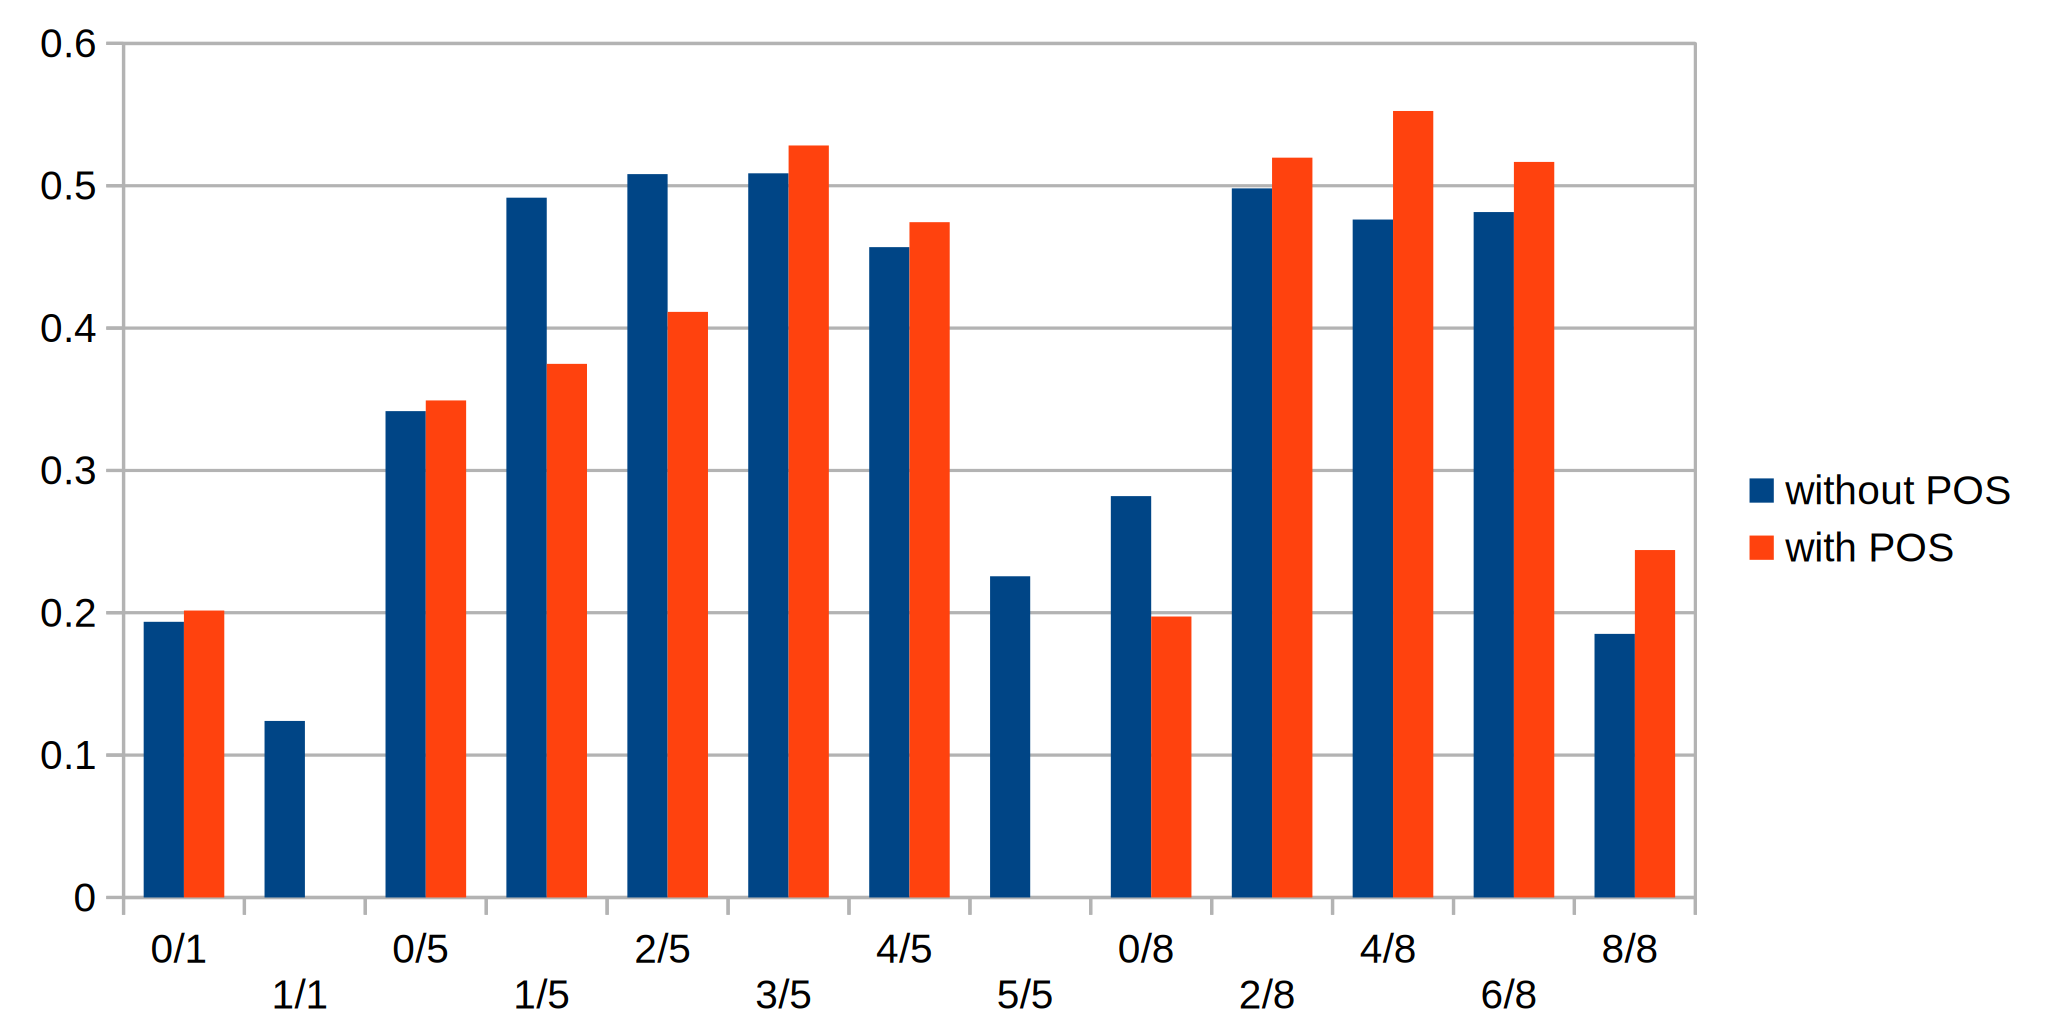
\includegraphics[width=0.9\textwidth]{img/window_eval.png}
    \caption{Harmonic mean between all F1 scores for all classes. \emph{2/5} means window size of five and punctuation position two. If \emph{wi} is in the label, it uses wikipedia training data.}
    \label{fig:window_eval}
\end{figure}

We did experiments do get relations between several parameters.
On the one hand we varied the window size and punctuation position.
In Figure \ref{fig:window_eval} you can see the results.
We found out that the best position for the punctuation is in the middle of the window.
We get the best results for a window size of 8.
This means that more context the better the results, until a certain point.

\begin{figure}[ht]
    \centering
    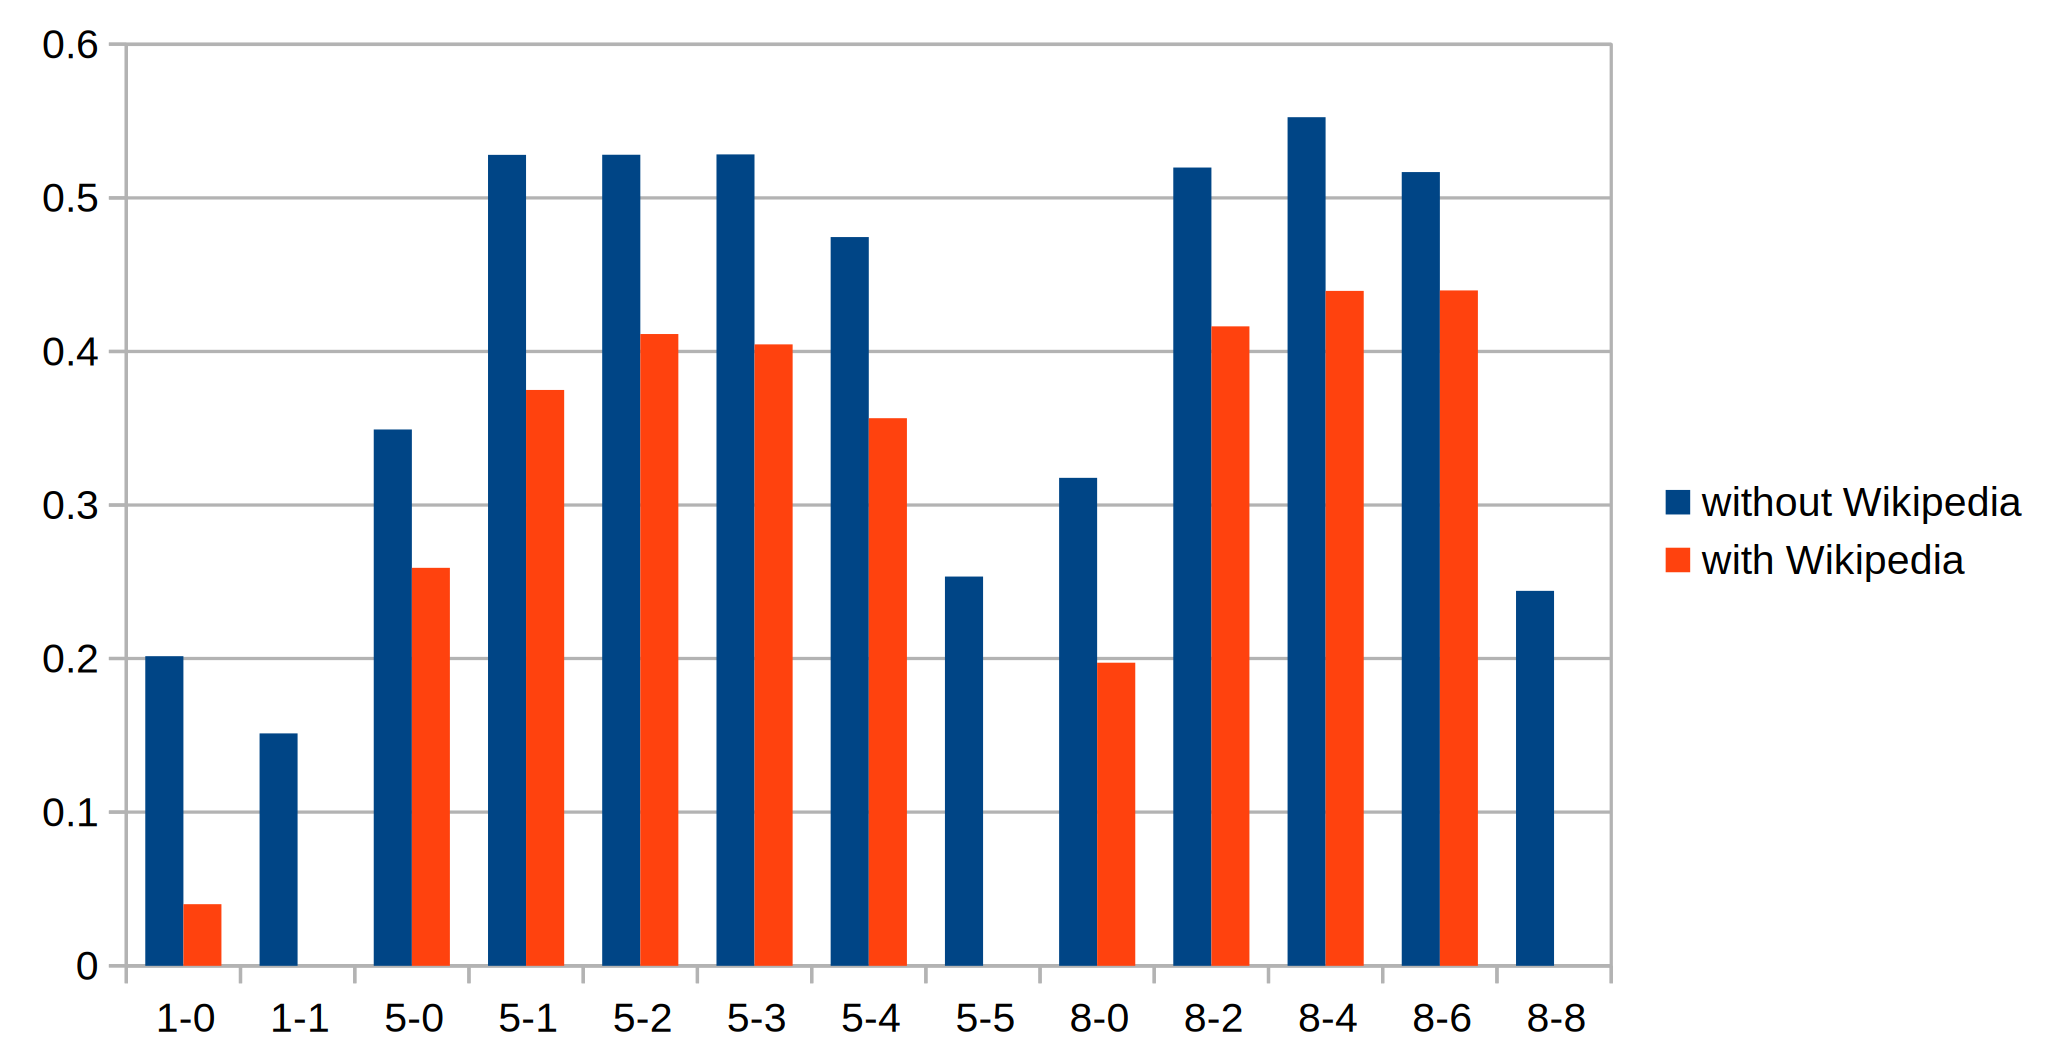
\includegraphics[width=0.75\textwidth]{img/window_wiki_eval.png}
    \caption{F score with different window and punctuation positions. Compares only TED talks and TED talks with additional wikipedia data as training data.}
    \label{fig:window_wiki_eval}
\end{figure}

As described in Section \ref{sec:training_data}, we wanted to use more data for lexical prediction.
In Figure \ref{fig:window_wiki_eval} a comparison between using only TED talks and using additionally wikipedia data as training data is shown.
The described F-score is used, as well as different window sizes and punctuation positions.
The result for varying the window size is the same as described in the experiments above.
You can see that using wikipedia data as additional training data always performs worse.
An experiment without wikipedia data has a F-score of 0.385, whereas the same experiment with wikipedia has only a F-score of 0.252.
This shows that more data does not help in general, although we think that the more data the network learned from the better the results should be.
This result can be explained with the used testing data.
The trained network is evaluated with TED talks.
This is spoken language and wikipedia articles are written language by its nature.
We evaluated the network also with wikipedia data (different from trainings data), which yields to a F-score of 0.60.
This shows that written and spoken language is different, so that predicting punctuations for other language structures does not work that good as for data with the same structure.

\begin{figure}[ht]
    \centering
    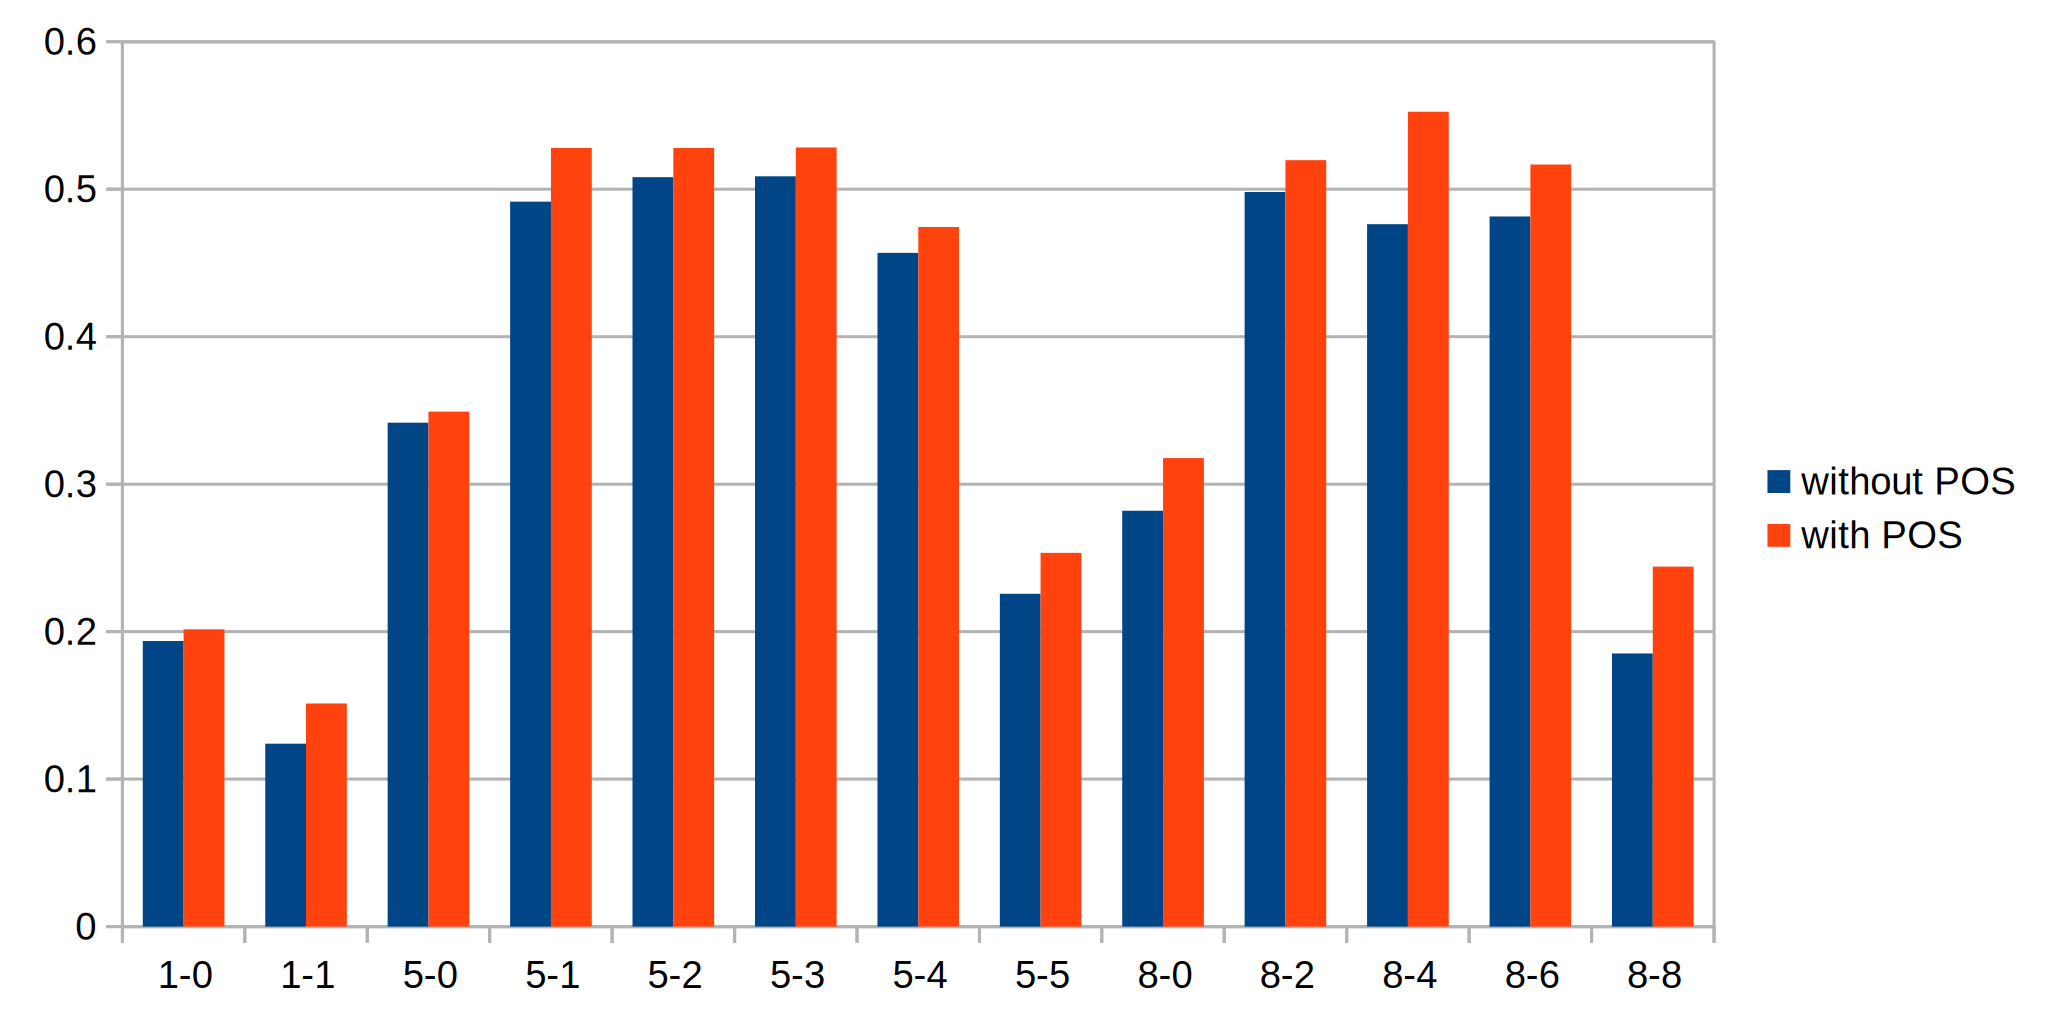
\includegraphics[width=0.75\textwidth]{img/window_pos_eval.png}
    \caption{}
    \label{fig:window_pos_eval}
\end{figure}

We also evaluated if using POS-Tags improves the results. Figure \ref{fig:window_pos_eval} shows the F-score depending on the different window sizes and punctuation positions. The red bars are the results with using the POS-Feature and the blue bars are the result without (the normals one, shown in the other graphs too).
You can see that using the additional POS Feature performs always better.
Compare to experiments with and without POS tagging (other than that, they have the same configurations) with POS tagging has a F-score of 0.305 whereas without POS tagging has only a F-score of 0.275.

Since the punctuation types in the data sets are not equally distributed, we thought about reducing the dataset to a set were the types are balanced. Therefore we created training sets, were nearly equally distributed punctuations types are included. Experiments show that this performs worse as the normal sets. This is likely since the data set is much smaller.
